\section{Služby komunikačních systémů -- obecný rozbor, signalizační systém SS7, Telecommunication Management Network -- TMN, telekomunikační služby z pohledu ekonomiky.}

\subsection{Služby komunikačních systémů}

Služby komunikačních systémů jsou funkce poskytované přes komunikační sítě a zařízení, které umožňují uživatelům komunikovat a vyměňovat informace.
Patří sem hlasové a~datové služby, SMS a~MMS, videohovory, VoIP, mobilní služby a další.
Jejich cílem je usnadnit komunikaci a~výměnu informací mezi uživateli.


\subsection{Telekomunikační služby}

Telekomunikační služby přenášejí informace pomocí signálů mezi koncovými zařízeními.

\subsubsection{Základní prvky}
\begin{itemize}
    \item
          \textbf{Vysílač}:
          příprava, zpracování a~vložení informace do~komunikačního kanálu pomocí signálu.
    \item
          \textbf{Přenosové médium}:
          prvky vytvářející přenosové prostředí pro~přenos informace v~požadované podobě signálu -- elektromagnetické, rádiové, kabelové, optické.
    \item
          \textbf{Přijímač}:
          příjem informace, signálu z~přenosového prostředí a~jeho zpracování pro předání cílovému subjektu.
\end{itemize}

\subsubsection{Kategorizace}
\begin{enumerate}
    \item Podle typu zpracování informace:
          \begin{description}
              \item[Analogové] Telefonní síť, terestiální analogové vysílání atp. (v~dnešní době postupně zanikající služby, nahrazované digitálními technologiemi).
              \item[Digitální] Datová síť.
          \end{description}
    \item Podle regulace:
          \begin{description}
              \item[Rezervované služby] Telefonní síť.
              \item[Oblasti regulované licenčními podmínkami] Televizní a~rádiové vysílání, mobilní komunikace.
              \item[Oblasti volného působení za~dodržení norem a předpisů] Služby uživatelského charakteru.
          \end{description}
    \item Podle potřeb uživatelů:
          \begin{description}
              \item[Základní a~rozšířené telefonní služby] Telefonní hovory, datové služby ISDN, doplňkové služby ke~zdokonalení základní služby (přenos telefonního čísla, volání na~účet volaného, roaming, SMS).
              \item[Telematické datové služby] Infrastruktura dopravy (navigační systémy, řízení dopravy).
              \item[Multimediální datové služby] IPTV, VoIP, internet, \dots; jsou kladeny vyšší nároky na~přenosová média z~hlediska zpracování a~rychlosti doručení informace.
          \end{description}
    \item Podle počtu současně komunikujících účastníků:
          \begin{description}
              \item[point to point] Komunikace pouze dvou uživatelů/bodů na~přenosovém médiu.
              \item[point to multipoint] Centralizované komunikace jednoho uživatele s~více: TV, IPTV, rozšířené telefonní služby a~rádiové vysílání, některé služby ISP.
              \item[multipoint to multipoint] Decentralizované komunikace: běžný internetový provoz.
          \end{description}
    \item Podle dosažitelnosti služeb:
          \begin{description}
              \item[Pevné] Digitální integrované služby ISDN, služby asynchronních sítí ATM, služby sítí LAN, služby internetového charakteru.
              \item[Mobilní] Služby bezdrátových paketových sítí, služby GSM standardů.
          \end{description}
\end{enumerate}

\subsection{Signaling System Number 7}

SS7 je sada signalizačních protokolů používaných v~mobilních telefonních sítích, pozemních digitálních telefonních sítích a pro mezi-ústřednovou signalizaci.
Úkolem SS7 je poskytovat informace k~navázání, uskutečnění a~ukončení telefonních hovorů a k~dalším službám (SMS, účtování, překlady telefonních čísel).


\subsubsection{Přenosová síť SS7}

SS7 síť se skládá z~různých uzlů:
\begin{description}
    \item[SSP \emph{(Service Switching Point)}]:
    telefonní ústředna zajišťující propojování hlasových spojení.
    U~mobilních stanic se používá název MSC \emph{(Mobile Switching Centre)}.
    \item[STP \emph{(Signal Transfer Point)}]:
    funkce routeru, tj. propojování SSP a SCP.
    \item[SCP \emph{(Service Control Point)}]:
    řízení služeb sítě (směrovací databáze) nutné pro~distribuci dat.
\end{description}

Jeden signalizační kanál SS7 je schopen obsloužit až tisíc kanálů přenášejících hlas nebo data.
VoIP a LTE již SS7 nepoužívají, protože byl nahrazen lepšími protokoly.

\subsubsection{Protokoly SS7}

Protokol \textbf{MTP} \emph{(Message Transfer Part)} se skládá ze~tří úrovní odpovídajícím fyzické, spojové a síťové vrstvě (MTP1, MTP2, MTP3).
Zástupci aplikačních protokolů jsou:

\begin{itemize}
    \item \textbf{MTP} \emph{(Message Transfer Protocol)}: přenos signalizace uvnitř národní sítě operátora.
    \item \textbf{SCCP} \emph{(Signaling Connection Control Part)}: směrování signalizačních zpráv dle~telefonních čísel; propojování operátorů a států.
    \item \textbf{TCAP} \emph{(Transaction Capabilities Application Part)}: výměna informací mezi sítí a ústřednami.
    \item \textbf{MAP} \emph{(Mobile Application Part)}: signalizace o~lokaci účastníků, přenos dat a~SMS, \dots
\end{itemize}


\subsection{Telecommunication Management Network}

TMN je koncept používaný pro~správu a monitorování telekomunikačních sítí.

\begin{itemize}
    \item \textbf{Business management}: plánování, strategie, marketing a řízení ekonomických výdajů.
    \item \textbf{Service management}: správa a řízení služeb poskytovaných koncovým uživatelům (správa služeb, řízení QoS, fakturace, reklamace).
    \item \textbf{Network management}: správa infrastruktury a sítí (konfigurace, monitoring, řízení chyb a bezpečnosti).
    \item \textbf{Element management}: správa prvků sítě (konfigurace, monitoring, diagnostika, řízení).
\end{itemize}


\subsection{Pohled ekonomiky}

Telekomunikace jsou páteří všech odvětví ekonomiky i dopravních systémů.
Je to zpravidla více služeb které vytvářejí podmínky k~řešení telekomunikační úlohy.

Náklady na~provoz a poskytování služeb jsou významné faktory omezující růst samotné infrastruktury, jejich služeb i oborů na~nich závislých.

Proto je velmi důležité sdílení kapacit linek mezi všemi subjekty.
Možnost sdílení je podmíněno zaručením bezpečnostní integrity jednotlivých aplikací.


\clearpage
\section{Integrované služby digitální sítě -- ISDN, základní a primární přístup, referenční model účastnické přípojky ISDN, strukturu rámce na rozhraní S a U, napájení terminálů.}

ISDN \emph{(Integrated Services Digital Network)} umožňovala přenos digitálních dat spolu s~digitalizovaným hlasem přes komutované okruhy veřejnou telefonní sítí.

Pro~přenos používala tzv. B-kanály \emph{(bearer)} s~přenosovou rychlostí 64~kbps, signalizační D-kanál měl rychlost 16~kbps.
H-kanály je spojení \emph{(bonding)} více (6, 23, 24, 30) datových B-kanálů.

\textbf{BRI} \emph{(Basic Rate Interface)} byl určen pro~individuální uživatele.
Skládal se z~dvou B-kanálů (pro~celkovou rychlost 128~kbps) a jednoho D-kanálu.
\textbf{PRI} \emph{(Primary Rate Interface)} byl určen pro~podniky.
Skládal se z~30 B-kanálů (pro~celkovou rychlost 2~Mbps) a jednoho D-kanálu.

\subsection{Referenční model}

\begin{figure}[ht]
    \centering
    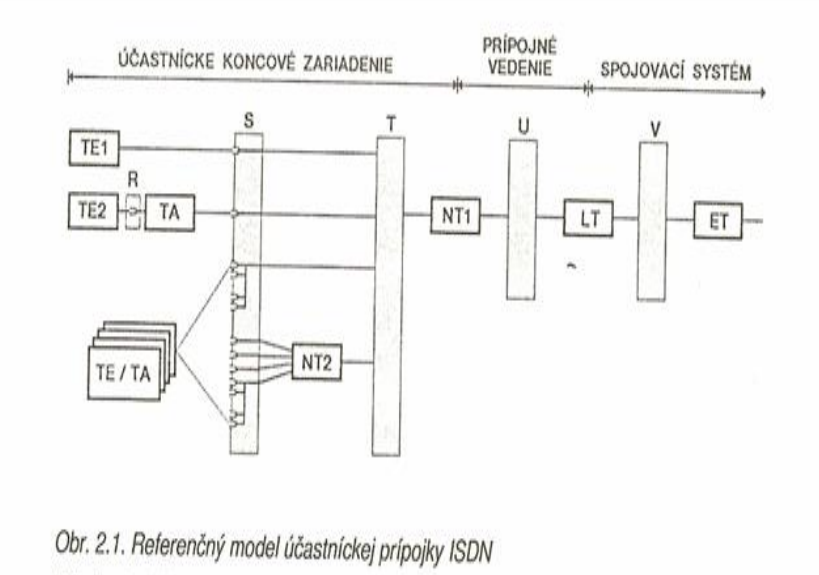
\includegraphics[width=0.75\textwidth]{snimky/ISDN-ref.png}
    \caption{
        Model ISDN.
        \\Rozhraní U je dvoudrát mezi telefonní ústřednou a~terminační jednotkou.
        \\Rozhraní T je sériová přípojka vedoucí k~terminálu (=modem).
        \\Rozhraní S je čtyřdrát odpovídající T.
        \\Rozhraní R je překlad mezi sítí a ne-ISDN zařízením.
    }
\end{figure}
\FloatBarrier


\subsubsection{Struktura rámce S}

Každý rámec obsahuje signalizační informace, pomocné bity, uživatelská data a~synchronizaci.

\begin{center}
    \begin{tabular}{cll}
        \textbf{bit} &                  & \textbf{popis}                    \\
        F            & \emph{framing}   & začátek rámce                     \\
        L            & \emph{balancing} & vyvážení stejnosměrné složky      \\
        D            & \emph{channel}   & bit D kanálu                      \\
        E            & \emph{echo}      & řízení přístupu stanic ke~kanálům \\
        S            & --               & budoucí použití                   \\
        A            & --               & protokoly aktivace                \\
        B1,B2        & --               & bity kanálů B1 a B2               \\
    \end{tabular}
\end{center}


\subsubsection{Struktura rámce U}

Kódování 4B/3T nebo 2B/1Q.


\subsection{Napájení terminálů}

Napájení terminálů v~ISDN bylo možné realizovat:

\begin{enumerate}
    \item \textbf{Interní napáječ terminálu}.
    \item \textbf{Síťový napáječ NT}: fantomní napájení skrz datový kabel.
    \item \textbf{Napájení z~jiného terminálu}: připojení pomocí přídavného páru vodičů a jednotky NT která umožňuje přenos napájení mezi terminály.
    \item \textbf{Napájení z~ústředny přes NT a rozhraní~S0}: fantomní napájení z~ústředny přes rozhraní S0.
\end{enumerate}


\clearpage
\section{Asynchronní přepravní způsob -- ATM, buňka ATM, synchronizace, virtuální cesta a virtuální kanál, třídy služeb, ATM vrstvový model, síťové prvky ATM.}

ATM je standard vytvořený pro~\enquote{vysokorychlostní} síťě 80. a~90.~let.
Má buňky o~konstantní velikosti (5+48~B) a podporuje QoS pro~přenos hlasu a videa.
Přenášeny jsou samostatné pakety směrovány dle jejich identifikátoru ve~virtuálním okruhu (sestaveném pro~celý přenos).

Mělo jít o~technologii nahrazující ISDN, ale místoho toho byl na~sítích nasazen rychlejší a~efektivnější Ethernet.


\subsection{Buňka v ATM}

Buňka mezi účastníkem a~sítí (UNI-ATM) a uvnitř sítě (NNI-ATM) se téměř neliší, jediné rozdílné pole nakonec nebylo využíváno.

\begin{figure}[h]
    \centering
    \onehalfspacing
    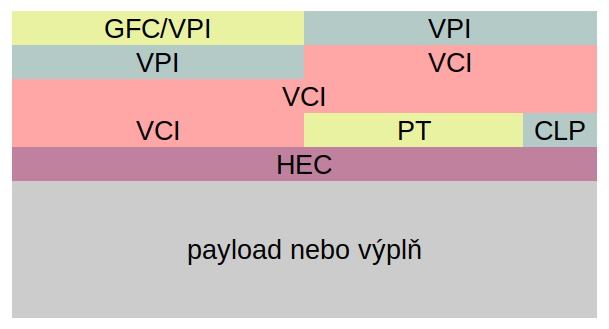
\includegraphics[width=0.5\textwidth]{snimky/atm-bunka}
    \caption{
        Schéma ATM buňky; šířka reprezentuje osm bitů. \\
        GFC \emph{(Generic Control Flow)}: pouze UNI-ATM, nevyužíváno,
        VPI \emph{(Virtual path identifier)},
        VCI \emph{(Virtual channel identifier)},
        PT \emph{(Payload type)}: network management, zahlcení, user--to--user;
        CLP \emph{(Cell loss priority)},
        HEC \emph{(Header error control)}: CRC.
    }
    \label{fig:atm-bunka}
\end{figure}


\subsection{Synchronizace}

Buňky jsou přenášeny neustále.
Pokud stanice nemá data k~odeslání, vysílají se prázdné buňky a tím se dosáhne plynulého toku dat.
Přenos jako takový je asynchronní.


\subsection{Virtuální cesty a kanály}

Jedna virtuální cesta (VP) může mít více virtuálních okruhů (VC).
Během přenosu buňky se hodnoty VPI a~VCI mění (tzv. \emph{label swapping}).

\begin{figure}[ht]
    \centering
    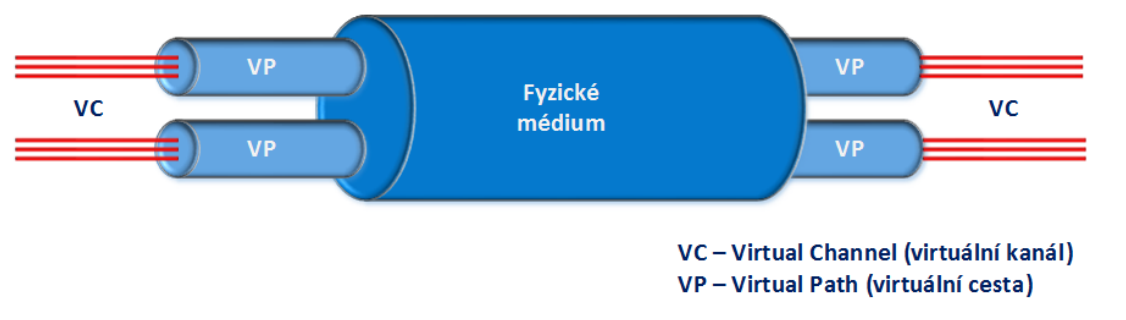
\includegraphics[width=0.8\textwidth]{snimky/VC.png}
    \caption{Vizualizace ATM spojení.}
    \label{fig:virt-cesty-kanaly}
\end{figure}
\FloatBarrier


\subsection{Třídy služeb}

Pro~zajištění QoS slouží čtyři třídy.

\begin{figure}[ht]
    \centering
    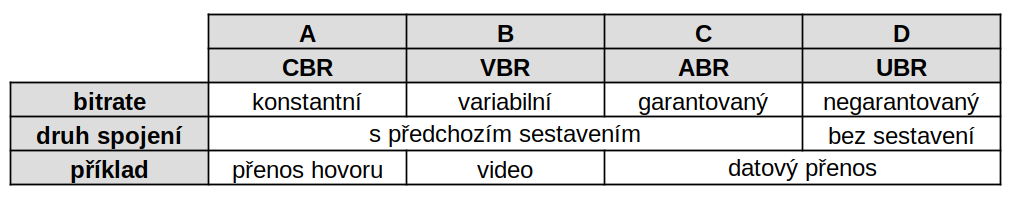
\includegraphics[width=0.8\textwidth]{snimky/atm-tridy}
    \caption{Třídy ATM provozu.}
\end{figure}
\FloatBarrier


\subsection{Vrstvový model ATM}

\textbf{Fyzická vrstva} se dělí na PMD (\emph{Physical Medium Dependent}; synchronizace) a TC (\emph{Transmission Convergence}; kontrola záhlaví buněk, směrování).

\textbf{ATM vrstva} poskytuje \emph{Generic Flow Control}, multiplexování a překlady VCI/VPI hodnot.

\textbf{Adaptační vrstva} přiděluje šířku pásma, poskytuje spojově orientovanou službu a provádí emulaci okruhů pro~aplikace (hlas, videokonference).


\subsection{Síťové prvky v~ATM}

V~síti ATM se vyskytují různé síťové prvky:
přepínače \emph{(switches)} přepínají buňky ATM mezi různými virtuálními cestami a~kanály,
směrovače \emph{(routers)} směrují datový provoz mezi různými sítěmi,
terminály \emph{(terminals)} slouží jako koncové body přenosu dat.


\clearpage
\section{Digitální účastnická přípojka xDSL, HDSL, ADSL, spojení, referenční model, modulace, rušivé vlivy, přeslechy.}

\subsection{xDSL -- Digital Subscriber Line}
Digitální účastnické přípojky jsou technologie pro rychlé připojení konečných uživatelů k poskytovatelům služeb využívající existující infrastrukturu, jako je telefonní síť.

Nejznámějšími typy xDSL (Digital Subscriber Line) jsou HDSL (High-bit-rate Digital Subscriber Line), ADSL(Asymmetric Digital Subscriber Line), VDSL (Very-high-bit-rate Digital Subscriber Line), atd. Každý typ xDSL má specifické frekvenční pásmo, přenosovou rychlost a dosah.

Obecně platí, že čím horším je vedení od ústředny k uživateli (kvalita rozvodu a délka), tím menší je přenosová rychlost. Nejčastějším typem DSL je stále ještě ADSL, postupně je však nahrazováno sofistikovanějšími a rychlejšími technologiemi \textbf{Is it really??}.

Jsou rozlišovány dvě základní verze xDSL technologie:
\begin{itemize}
    \item Symetrická -- symetrická řešení poskytují jak v dopředném, tak i v opačném směru synchronní přenos dat.
    \item Asymetrická -- ADSL, VDSL
\end{itemize}

\subsection{HDSL}
HDSL je jednou z technologií xDSL, která se používá pro přenos dat vysokou rychlostí po telefonních linkách. HDSL je symetrická technologie, což znamená, že nabízí stejnou rychlost pro stahování i nahrávání. Byla představena na trhu v 90. letech jako součást digitálního vývoje telefonních připojení. HDSL je navrženo pro podnikové prostředí a umožňuje dosáhnout rychlostí až 1,544 Mbps nebo 2,048 Mbps na jedné telefonní lince.

\subsection{ADSL}
ADSL je asymetrická xDSL technologie, která umožňuje rychlé připojení k internetu a přenos dat po telefonních linkách. Byla představena na trhu v 90. letech jako způsob využití stávající telefonní infrastruktury pro poskytování širokopásmového připojení. ADSL je asymetrické, což znamená, že nabízí vyšší rychlost stahování dat než rychlost nahrávání. Typické rychlosti ADSL se pohybují od 8 Mbps do 24 Mbps pro stahování a od 1 Mbps do 3 Mbps pro nahrávání. Tato technologie je vhodná pro domácnosti a malé firmy, které potřebují přístup k internetu a online službám.

\subsection{Spojení a referenční model}
\begin{figure} [h]
    \centering
    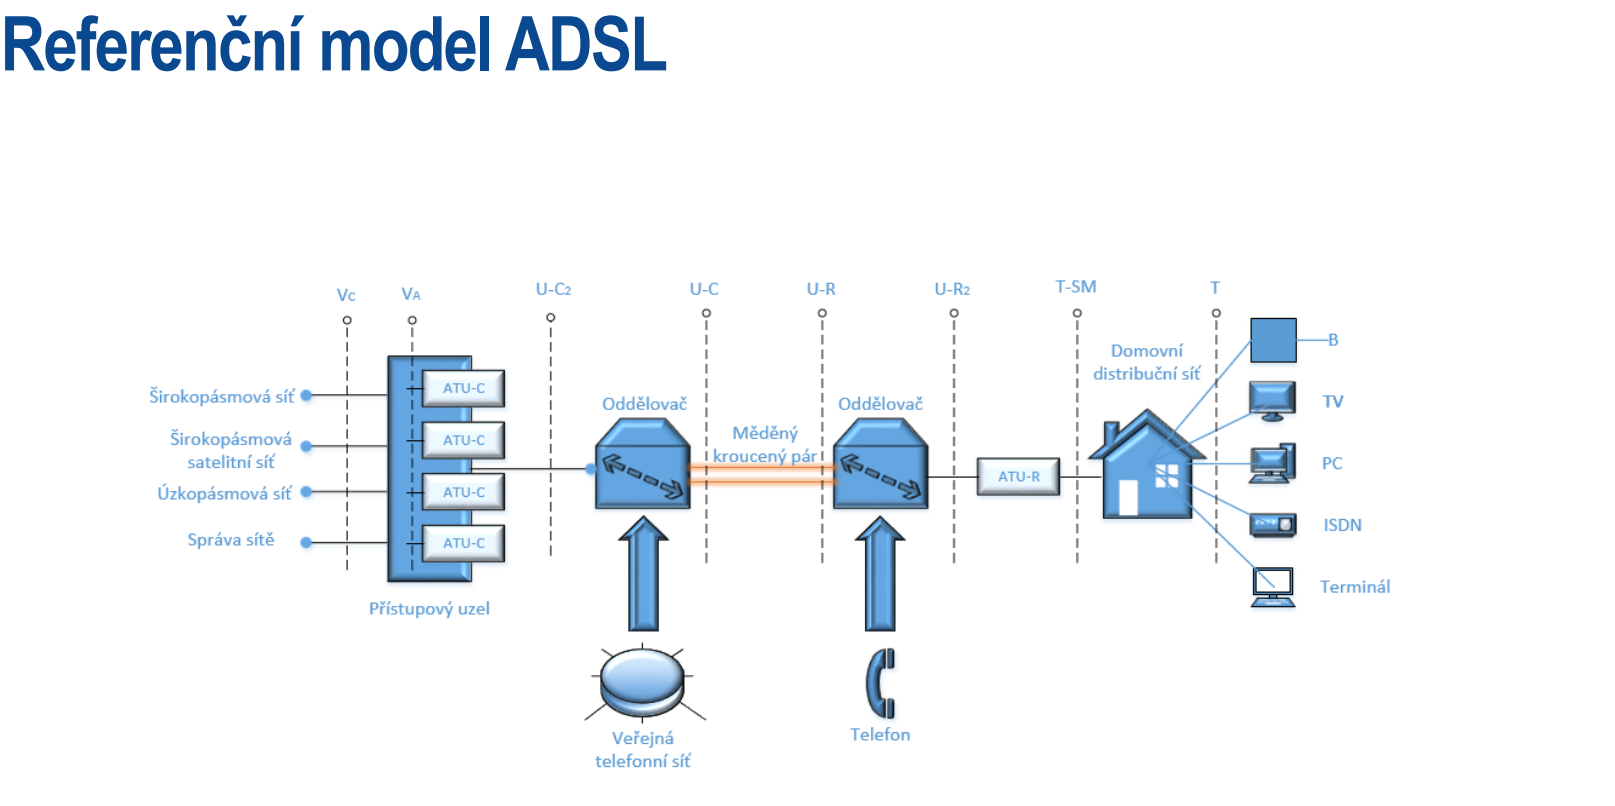
\includegraphics[scale=0.85]{snimky/ADSL model.png}
\end{figure}
\newpage
\subsubsection{Spojení (asi myslel zapojení...)}
\begin{figure} [h]
    \centering
    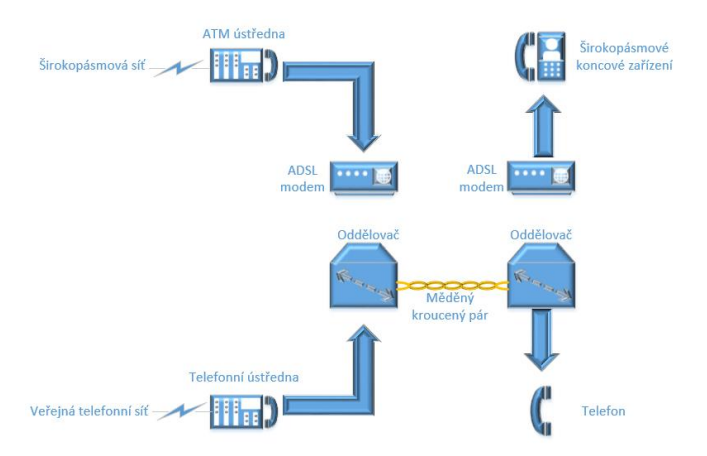
\includegraphics[scale=0.8]{snimky/zapoj.png}
\end{figure}

Hlavní komponenty sítě:
\begin{itemize}
    \item DSLAM (DSL Access Multiplexer) -- slučuje hlasový provoz a DSL provoz na jednu telefonní linku (dvoudrát),pracuje na L2 vrstvě jako switch, funkce tzv. přístupového koncentrátoru, k jednomu DLSAMu lze připojit až několik tisíc uživatelů, záleží na počtu portů dané karty.
    \item ADSL modem -- modem pro přípojku, k PC se připojuje přes Ethernet, popř. USB.
\end{itemize}

\subsubsection{Modulace}
Využíva se kvadraturní amplitudová modulace QAM, amplitudová fázová modulace bez nosné CAP, diskrétní vícetónová modulace DMT.
\begin{itemize}
    \item \textbf{QAM} -- používaná ve velké řadě aplikací (např. modemy v základním pásmu, mikrovlnné radiové systémy aj.). Modulace se provádí pomocí digitálního kvadraturního (ortogonálního) modulátoru se sinusovou a kosinusovou směšovací funkcí. Díky této ortogonalitaě (nosných signálů) se umožní následná detekce dat v přijímači.
    \item \textbf{CAP} -- podobná QAM. Používá stejné dvourozměrné přenosové schéma a má stejný typ výkonového spektra. Modulace se provádí pomocí digitálních transverzálních pásmových filtrů. Impulsní odezva těchto filtrů má stejnou amplitudovou charakteristiku, ale fázová charakteristika se navzájem liší o 90°.
    \item \textbf{DMT} -- jeví se v systémech ADSL jako velmi perspektivní a výrobci podporovaná. Modulace s více nosnými MCM. Je založena na diskrétní Fourierově transformaci, resp. na rychlé Fourierově transformaci FFT (Fast Fourier Transform). Velkou výhodou této metody modulace je plně digitální realizace a poměrně nízká složitost. Pomocí DMT lze efektivněji řešit negativní vlivy nedokonalé přenosové cesty a také rušící vliv okolí na užitečný signál při přenosu symetrickým párem v metalické přístupové síti
\end{itemize}
\newpage

\subsubsection{Rušivé vlivy}
\begin{figure} [h]
    \centering
    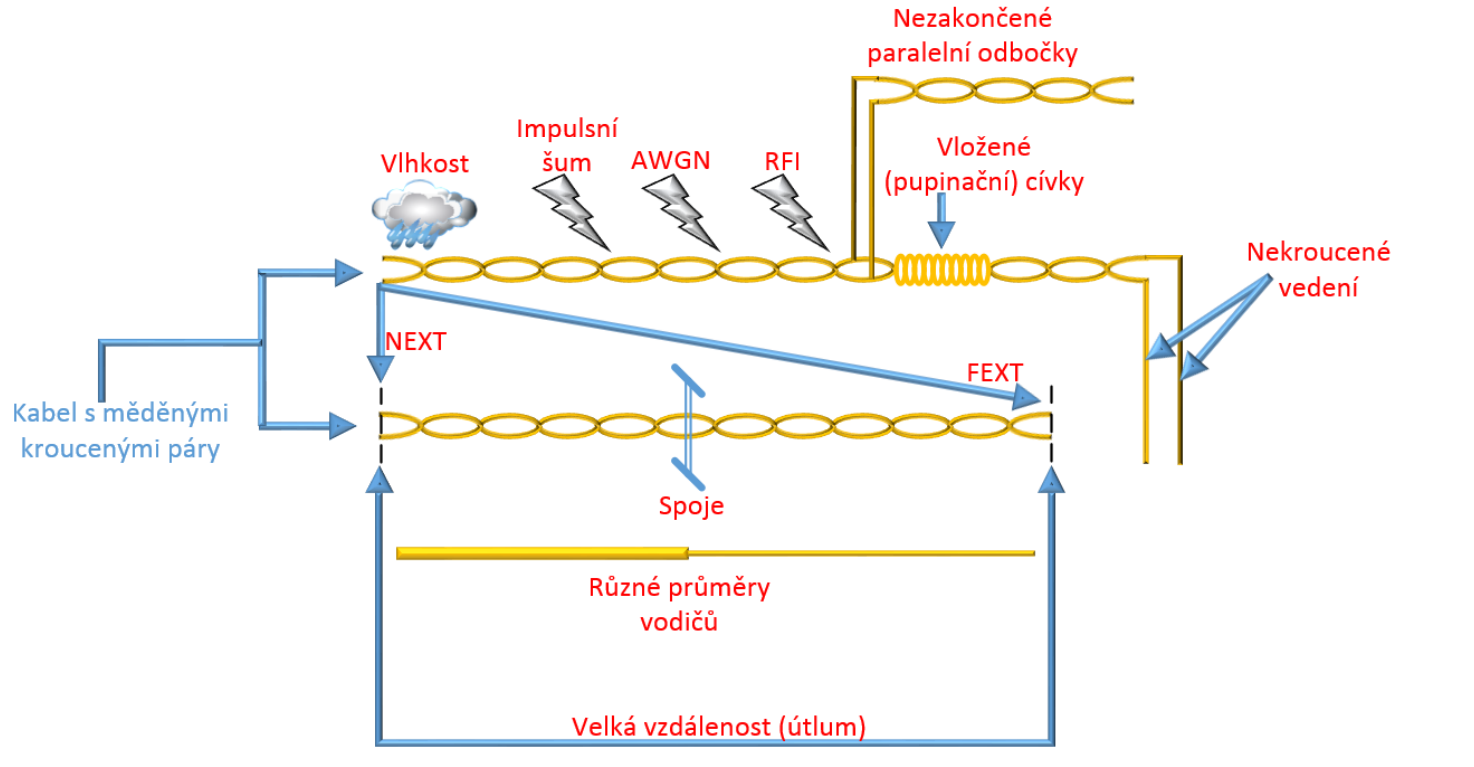
\includegraphics[width=0.8\textwidth]{snimky/ADSL ruch.png}
    \label{fig:adsl-ruch}
\end{figure}
\begin{itemize}
    \item Vnější rušivé vlivy
    \item Impulsní rušení -- impulsive noise
    \item Vf rušení -- RFI (Radio Frequency Interference)
    \item Vnitřní rušivé vlivy
    \item NEXT (Near End cross talk)
    \item FEXT (Far End cross Talk)
    \item AWGN (Additive White Gausian Noise)
\end{itemize}

\subsubsection{Přeslechy}
NEXT, FEXT
Aditivní bílý šum (Tepelný šum, Výstřelový šum, Kvantizační šum, Zbytkový odrazový šum)


\subsubsection{Metody zabezpečení proti chybám v DSL}
\begin{itemize}
    \item Detekce chyb pomocí cyklického kódu CRC
    \item Dopředná chybová korekce FEC -- Spolu s prokládáním poskytuje FEC ochranu hlavně proti shlukům chyb. Skramblování neslouží k opravě chyb, ale rozrušuje dlouhé posloupnosti jedniček a nul a tak zabezpečí lepší synchronizaci na přijímací straně.
    \item Interleaving -- ochrana zabezpečení dat při přenosu v prostředí, zarušené především impulsním šumem. Zvyšuje odolnost přenosu, ale vnáší do přenosu větší zpoždění.
\end{itemize}


\clearpage
\section{IPv6, návaznost na IPv4, kvalita služeb QoS, referenční model OSI versus síťová architektura TCP/IP.}


\subsection{IPv6}

IPv6 je protokol síťové vrstvy modelu TCP/IP.
Adresy mají délku 128 bitů (proti 32 bitům ve~IPv4) a nabízí tak nevyčerpatelný prostor adres (matematicky $10^{39}$ použitelných adres, zhruba $6 \cdot 10^{19}$ na~každý~cm$^2$ povrchu Země).
Obě verze v~současném internetu koexistují (tzv. \emph{dual stack}) a je nutné provádět duální konfigurace (směrování, firewally, DNS).

IPv6 hlavička má pouze 40~bajtů, protože byla odstraněna nepoužívaná pole z~hlavičky IPv4.
Poli v~IPv6 jsou: verze IP, třída provozu, identifikace toku dat, délka datagramu, další záhlaví/identifikátor vyšší vrstvy, limit počtu skoků, zdrojová a~cílová adresa a přenášená data.

Směrování je v~IPv6 beztřídní, stejně jako v~současných verzích IPv4.
Podporuje tři typy adres: \underline{unicast} jsou adresy konkrétních rozhraní zařízení, \underline{anycast} jsou speciální adresy které jsou sdílený více zařízeními, ale provoz je směrován pouze jednomu z~nich (nejčastěji geograficky nejbližšímu) a \underline{multicast} jsou vícesměrové adresy na~kterých naslouchá více zařízení.
V~IPv4 navíc existují broadcast adresy které reprezentují všechny adresy v~dané síti.


\subsection{Quality of Services}

Kvalita služeb je metrika propustnosti a~efektivnosti sítí a služeb.
K~základním měřeným parametrům patří:
\begin{itemize}
    \item komunikační zpoždění: packetové, rámcové, způsobené kódováním,
    \item jitter: odchylka zpoždění jednotlivých rámců,
    \item šířka pásma: kapacita linky,
    \item ztrátovost: zastoupení nedoručených datagramů způsobené rušením linky nebo zahlcením síťových prvků,
    \item míra pravděpodobnosti blokování: čekání ve~frontách.
\end{itemize}

Dále může být provoz měřen objektivními a subjektivními testy, které se měří a vyjadřují v~jednotkách MOS \emph{(Mean of Service)} a které reprezentují vnímání kvality služby uživatelem.

V~IPv4 bývá častým zdrojem latence fragmentace paketů.
IPv6 tento problém limituje zákazem fragmentace na~úrovni směrovačů (pakety překračující MTU jsou zahozeny).


\subsubsection{Služby}

\underline{\emph{Best Effort}} jsou služby s~negarantovaným doručením.
Síťové prvky se maximálně snaží o~jejich doručení, ale při~zahlcení mohou být zahozeny.
Směrovací prvky je typicky uschovávají ve~frontách FIFO \emph{(First In, First Out)}, ve~kterých čekají dokud na~ně nedojde řada.

\underline{IntServ} \emph{(Integrated Services)} rezervují kvalitu služeb pro~celou dobu trvání přenosu (tj. budují okruhy).
Aplikace si samy určují nároky na~svůj přenos, který ukládají do~datagramu kde jej mohou směrovače přečíst.
IPv4 i IPv6 sítě k~tomu mohou používat RSVP \emph{(Resource Reservation Protocol)}.

\underline{DiffServ} \emph{(Differentiated Services)} používá k~určení QoS směrovače na~základě klasifikace přenosu, ne vysílací stanice.
Využívají se metody jako WFQ \emph{(Weighted Fair Queuing)} nebo WRED \emph{(Weighted Random Early Detection)}.


\subsection{Referenční model OSI}

ISO/OSI je teoretický model struktury počítačových sítí, který předpokládá jednoduché terminály.
Obsahuje sedm vrstev s~pevně stanovenými úkoly.

\begin{enumerate}
    \item
          Fyzická vrstva:
          zajišťuje spojení mezi zařízeními na~fyzické úrovni a transformuje digitální signál na~impulsy na~fyzickém médiu.
          Základní jednotkou je bit.
    \item
          Linková vrstva:
          zajišťuje přenos a~zpracování rámců v~rámci segmentu.
          Zajišťuje bezporuchovou službu a~vytvoření zdálnivě kontinuální spojení mezi dvěma síťovými prvky.
    \item
          Síťová vrstva:
          zajišťuje směrování paketů co nejvhodnější cestou v~síti.
    \item
          Transportní vrstva:
          zajišťuje řízení komunikace mezi odesílatelem a~příjemcem a poskytuje přenos a~zpracování TCP/UDP segmentů/datagramů.
    \item
          Relační vrstva:
          zajišťuje navázání, udržování a ukončení relací mezi účastníky spojení.
    \item
          Prezentační vrstva:
          zajišťuje kódování, překlad, konverzi, šifrování a kompresi přenášených dat.
    \item
          Aplikační vrstva:
          provádí správu aplikačních systémů a~programů.
\end{enumerate}
\FloatBarrier


\subsection{Porovnání ISO/OSI a TCP/IP}

\begin{table}[ht]
    \centering
    \begin{tabular}{lll}
        \textbf{ISO/OSI}   & \textbf{TCP/IP}          & zástupci                        \\
        \hline \hline
        aplikační vrstva   & aplikační vrstva         & HTTP, DNS                       \\
        prezentační vrstva &                          &                                 \\
        relační vrstva     &                          &                                 \\
        \hline
        transportní vrstva & transportní vrstva       & TCP, UDP                        \\
        \hline
        síťová vrstva      & internetová vrstva       & IP                              \\
        \hline
        spojová vrstva     & vrstva síťového rozhraní & 802.3 (Ethernet), 802.11 (WiFi) \\
        fyzická vrstva     &                          &                                 \\
    \end{tabular}
    \label{Srovnání modelů ISO/OSI a TCP/IP}
\end{table}


\clearpage
\section{Pasivní optické sítě (topologie sítě a způsob komunikace sestupný/vzestupný směr).}
Pasivní optické sítě (PON) se skládají z:
\begin{itemize}
    \item OLT -- je řídící jednotka, která řídí celou funkcionalitu PON pro obousměrnou komunikaci.
    \item ONU -- optická síťová jednotka realizující převod z optického signálu na elektrický signál nebo naopak.
    \item Splitter -- rozděluje optický signál na více signálů
\end{itemize}
\begin{figure} [h]
    \centering
    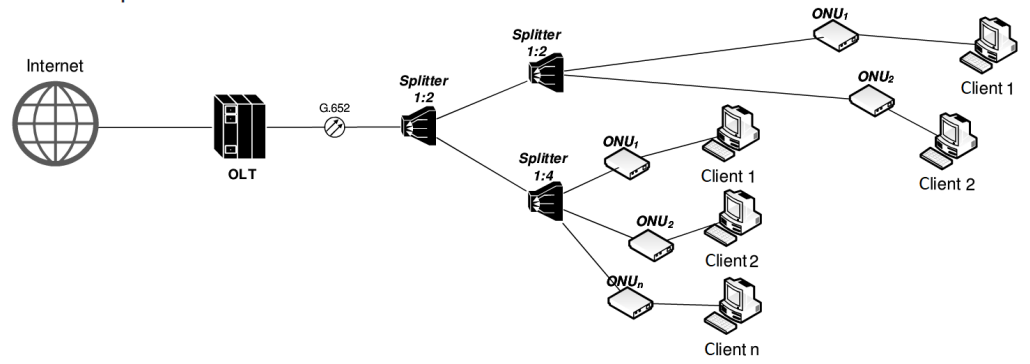
\includegraphics[width=\textwidth]{snimky/PONTopologie.png}
    \label{fig:pon}
\end{figure}

Komunikace probíhá v sestupném směru jako broadcast, kdy splitter dělí sestupný signál dle daného dělicího poměru (1:N) ke všem koncovým jednotkám ONU v poměru. ONU jednotka přijatý provoz filtruje na základě ONU-ID a cizí provoz je zahazován. Ve vzestupném směru mají jednotky dohodnutá časová okna ve kterých vysílají (TDM). Na základě potřeby vyšších rychlostí může docházet k úpravě délky těchto oken (např. algoritmus Max-Min Fair DBA).

\begin{figure} [h]
    \centering
    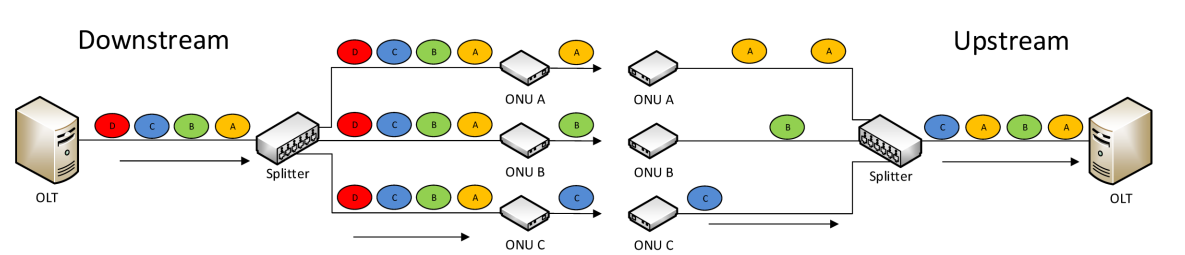
\includegraphics[width=\textwidth]{snimky/upDownPON.png}
\end{figure}

Pro realizaci obou směrů na jednom vlákně je využito dělení podle času (TDM) a vlnové délky (WDM). Pro downstream je dělení pomocí WDM -- rozdílná vlnová délka pro upstream oproti downstreamu, viz otázka 7. Pro upstream je komunikace koncových zařízení zajištěna pomocí časového multiplexu.

\clearpage
\section{Vývoj pasivních optických sítí a jejich rozdíly z pohledu fyzické a přenosové vrstvy.}

\subsection{ATM PON (APON) a BPON}
Rychlost v symetrické variantě 155,52\,MB/s a v asymetrické 622,8/155,52\,MB/s. BPON bylo pouze rozšíření a zvyšovala symetrickou rychlost na 622.8\,MB/s a přidávala nové funkce jako dynamickou distribuci pásma, vlnový multiplex (WDM). Používá ATM buňky.

\subsection{GPON}
GPON je nejpoužívanější v ČR. Využívá linkový kód NRZ (Non-return-to-zero) a podporuje plně ethernetové rámce se zapouzdřením do rámců GEM (Gigabit Passive Optical Network Encapsulation Mode) viz obrázek. Přenosové rychlosti závisí na použité variantě (symetrická/asymetrická).

\begin{figure} [h]
    \centering
    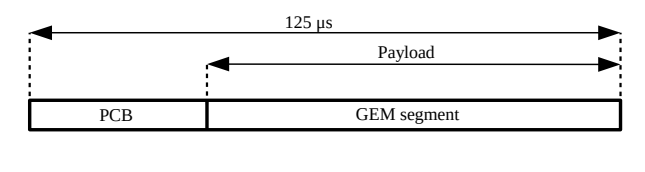
\includegraphics[width=\textwidth]{snimky/gemFrame.png}
\end{figure}

\subsection{EPON}
Odvozen od standardního Ethernet protokolu. Využívá linkový kód 8B/10B, tj. ke každému bloku 8 bitů jsou přidány 2 paritní bity. Pro přenos se využívá Ethernet rámců viz obrázek. Předchází kolizi paketů v síti pomocí MPCP (MultiPoint Control Protocol). Funguje na principu detekce ONU a ustanovení provozních parametrů, kdy na konci je mu přiděleno LLID. Primární rozmach měl na asijském trhu.

\begin{figure} [h]
    \centering
    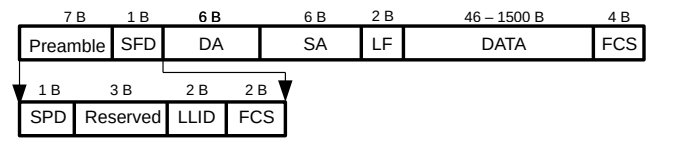
\includegraphics[width=0.8\textwidth]{snimky/EPONframe.png}
\end{figure}

\begin{itemize}
    \item SPD obsahuje informace o hodinovém signálu
    \item Reserved jsou tři byty pro budoucí účely
    \item LLID je identifikátor ONU
    \item FCS -- informace o detekci chyb
\end{itemize}

\clearpage

\begin{table}[ht]
    \centering
    \caption{GPON vs EPON (nevím jestli je ta přenosová vrstva správně)}
    \begin{tabular}{|l|l|l|}
        \hline
                                     & GPON           & EPON           \\\hline\hline
        \textbf{Fyzická vrstva}      &                &                \\\hline\hline
        Downstream [Gb/s]            & 1,244/2,488    & 1,25           \\\hline
        Upstream [Gb/s]              & 1,244/2,488    & 1,25           \\\hline
        Downstream vlnová délka [nm] & 1480\,--\,1500 & 1480\,--\,1500 \\\hline
        Upstream vlnová délka [nm]   & 1260\,--\,1360 & 1260\,--\,1360 \\\hline\hline
        \textbf{Přenosová vrstva}    &                &                \\\hline\hline
        Protokol                     & GEM            & Ethernet       \\\hline
        Linkové kodovaní             & NRZ            & 8B/10B         \\\hline
        Zabezpečení                  & downstream     & obousměrně     \\\hline
        Max dělící poměr             & 1:64           & 1:32           \\\hline
        Max dosah sítě [km]          & 20             & 20             \\\hline
    \end{tabular}
\end{table}

\subsection{XG-PON a XG(S)-PON}

XG-PON vylepšuje GPON, hlavně v nově použitém protokulu XGEM.

XGS-PON je pouze rozšíření XG-PON, kdy hlaví změnou je nově navržená TC (Transmission Convergence) vrstva, která je odvozena od standardu NG-PON2.

\subsection{10G-EPON}

Navazují standard na EPON s cílem možnosti provozovat 10G-EPON v souběhu s EPON na stejné optické distribuční síti. Používá Ethernet rámce. Existují ještě varianty 25G-EPON a 50G-EPON. Všechny jsou zpětně kompatibilní až po EPON.

\subsection{NG-PON2}
Poslední kompletně standardizovaný standard pro PON.

NG-PON2 umožnuje rychlost 40\,Gb/s s možností škálování až k hranici 80\,Gb/s. Využívá TWDM. TWDM pro vzestupný směr využívá tří typů pásem 1524-1544 (široké), 1528-1540 (zúžené) a 1532-1540 (úzké).

\begin{table}[ht]
    \centering
    \caption{XG(S)-PON vs 10G-EPON vs NG-PON2}
    \begin{tabular}{|l|l|l|l|}
        \hline
                                     & XG(S)-PON      & 10G-EPON       & NG-PON2                            \\\hline\hline
        \textbf{Fyzická vrstva}      &                &                &                                    \\\hline\hline
        Downstream [Gb/s]            & 9,9533         & 10,3125        & 40                                 \\\hline
        Upstream [Gb/s]              & 2,4883(9,9533) & 10,3125        & 10(asymetrický)/40(symetrický)     \\\hline
        Downstream vlnová délka [nm] & 1575\,--\,1580 & 1575\,--\,1580 & 1596\,--\,1603                     \\\hline
        Upstream vlnová délka [nm]   & 1260\,--\,1280 & 1260\,--\,1280 & 1524/1528/1533\,--\,1544/1540/1540 \\\hline\hline
        \textbf{Přenosová vrstva}    &                &                &                                    \\\hline\hline
        Protokol                     & XGEM           & Ethernet       & XGEM                               \\\hline
        Linkové kodovaní             & NRZ            & 64B/66B        & NRZ                                \\\hline
        Zabezpečení                  & obousměrně     & obousměrně     & obousměrně                         \\\hline
        Max dělící poměr             & 1:64           & 1:32           & 1:64                               \\\hline
        Max dosah sítě [km]          & 20             & 20             & 20                                 \\\hline
    \end{tabular}
\end{table}

\subsection{Super-PON}
\begin{itemize}
    \item Zvyšuje počet připojených ONU k jediné OLT z 64 na 1024
    \item Dochází ke snížení počtu CO, protože dosah sítě je zvýšen z 20 na 50 km
    \item Nasazení od 10 Gbit/s po 25 Gbit/s --> využití pro sítě 5G
    \item Používá Ethernet rámce
\end{itemize}

\subsection{Higher Speed PON (HSP)}
Parametry:
\begin{itemize}
    \item Přenosová rychlost -- sestupný směr: 49,77 Gbit/s
    \item Přenosová rychlost -- vzestupný směr: 49,77/24,88/12,44 Gbit/s
    \item Samo opravný kód: LDPC (low-density parity check)
    \item Linkový kód: NRZ
    \item Maximální vzdálenost přenosu: 20--40km
    \item Použitá vlnová délka 1340--1344nm
\end{itemize}

\begin{figure}[h]
    \centering
    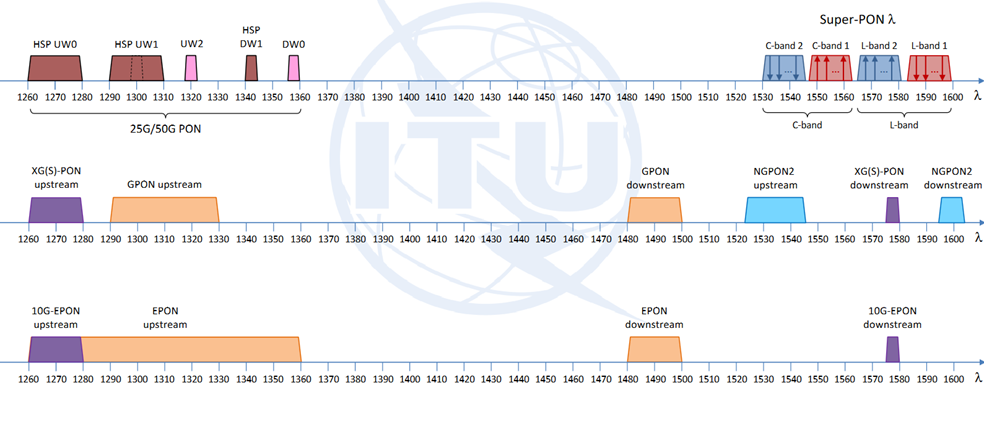
\includegraphics[width=\textwidth]{snimky/pon-kompatibilita.png}
    \caption{Kompatibilita PON protokolů}
\end{figure}

\clearpage
\section{Aktivační proces koncové jednotky v síti GPON.}
V současné době je GPON jedním z nejslibnějších řešení pro přístupové sítě (z pohledu ceny). GPON byl první standard, který podporoval přenos/zapouzdření ATM buněk i Ethernet rámců.

Aktivační proces:
\begin{figure} [h]
    \centering
    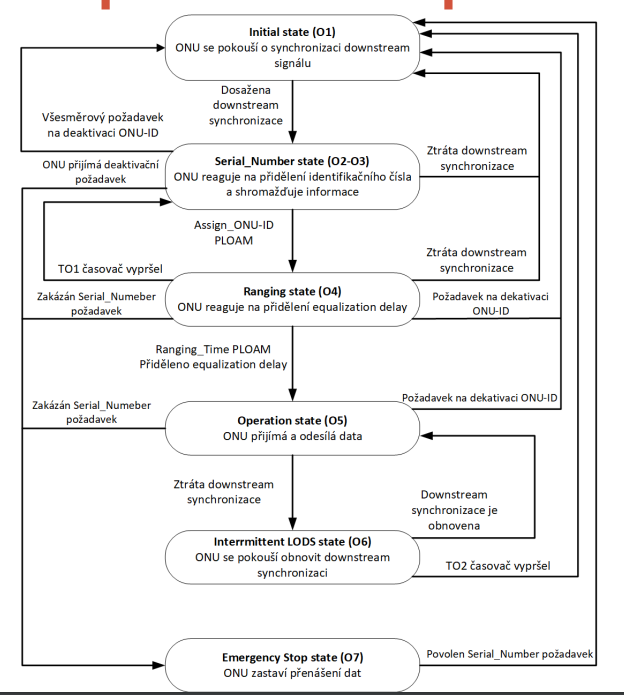
\includegraphics[width=0.63\textwidth]{snimky/proces.png}
    \label{fig:gpon-proces}
\end{figure}

Jednotka ONU komunikuje s OLT pomocí PLOAM zpráv, kdy typy zpráv a průběh komunikace je vidět níže.

\begin{figure} [h]
    \centering
    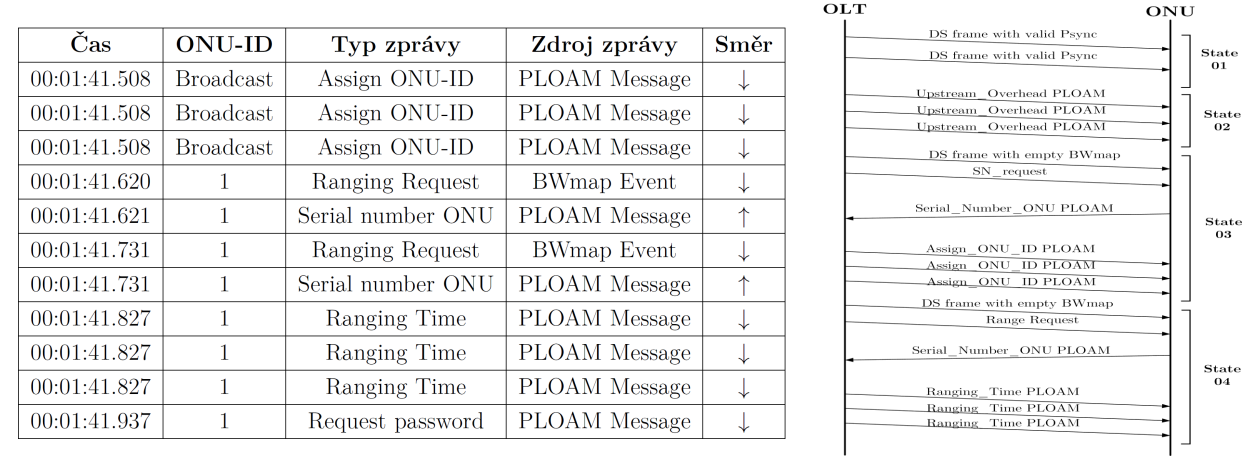
\includegraphics[width=0.9\textwidth]{snimky/aktivaceONU.png}
\end{figure}


\clearpage
\section{Využití celočíselného programování v současných sítích, síť jako graf, rozdělení zátěže z pohledu ceny přenosu.}
\textbf{Lineární programování} je obor matematiky, stejně jako matematika sama. \textbf{Lineární program} je maximalizace nebo minimalizace lineární funkce podléhající lineárním omezením (např. Lineární rovnice nebo lineární nerovnosti). Optimalizační problém s funkcí, která má být maximalizována nebo minimalizována, se nazývá \textbf{matematický program}. Pokud jsou proměnné v matematickém programu omezeny na nezáporná celá čísla, matematický program se nazývá \textbf{celočíselný program}.

\textbf{Realizovatelným/možným řešením} je řešení lineárního programu, které splňuje všechny omezení. Sada všech možných řešení se nazývá prostor pro řešení. Jestli že má lineární program realizovatelné řešení tak říkáme že je proveditelné jinak je neuskutečnitelné.

\subsection{Maximalizace toku, minimalizace ceny}

Maximalizace hledá tok v~orientovaném grafu tak, aby se maximalizoval objem přenosu ze~zdroje do~cíle při~dodržení kapacity spojů:
$\text{max}~v$.

Minimalizace hledá tok v~váženém orientovaném grafu tak, aby se při~maximálním objemu minimalizovala cena:
$\text{max}\ 4x_{12} + 8x_{13} + 2x_{23} + 6x_{24} + 7x_{34}$.

\begin{center}\begin{minipage}{0.3\textwidth}
        \begin{align}
            x_{12} + x_{23}          & = v     \\
            x_{12} - x_{23} - x_{24} & = 0     \\
            x_{13} + x_{23} + x_{34} & = 0     \\
            0 \leq x_{12}            & \leq 14 \\
            0 \leq x_{13}            & \leq 15 \\
            0 \leq x_{23}            & \leq 4  \\
            0 \leq x_{24}            & \leq 10 \\
            0 \leq x_{34}            & \leq 18
        \end{align}
    \end{minipage}\end{center}

\begin{figure}[ht]
    \centering
    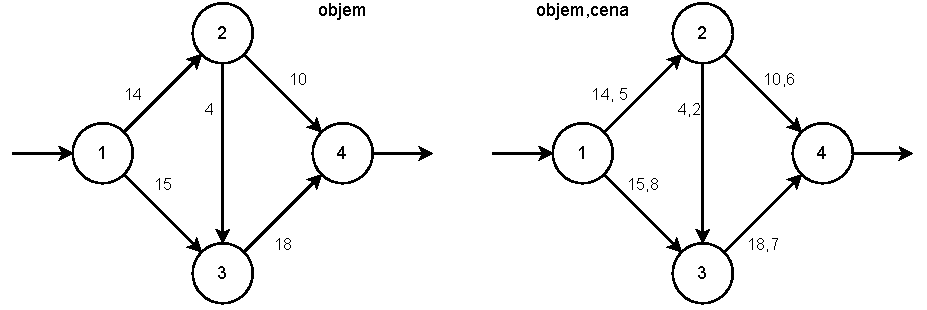
\includegraphics[width=\textwidth]{snimky/ilp}.
    \caption{Orientovaný graf (maximalizace toku) a vážený orientovaný graf (minimalizace ceny).}
\end{figure}


\clearpage
\section{IP přenos sítí wavelength division multiplexing (WDM), CWDM, DWDM, TDM versus WDM, problematika přiřazování vlnových délek (RWA).}

\subsection{Vlnový multiplex WDM}

Přenos více signálů jedním optickým vláknem v rozdílných vlnových délkách. Je základem pro všechny rozšiřující vlnové multiplexy. Klasické WDM pomocí multiplexoru přidávalo k signálu jednu další nosnou vlnovou délku. Pomocí demultiplexoru je následně signál opět rozdělen.

\subsubsection{IP přes WDM}

Slouží k přenosu IP protokolu v optické síti s podporou WDM. IP jako technologie síťové vrstvy spoléhá na vrstvu datového spojení poskytující rámcování, detekci chyb, obnovení chyb (opakování požadavku při chybě). Motivace pro IP/WDM může být, že za využití stávající infrastruktury, lze pomocí WDM zvýšit šířku pásma vláken. Většina přenosů mezi sítěmi využívá IP a zároveň většina uživatelských aplikací podporuje IP.

\subsection{Vlnový multiplex CWDM }
Označovaný jako \enquote{hrubý}, umožňuje v jediném optickém vlákně přenášet najednou až 18 nezávislých optických signálů s různou vlnovou délkou. Každý přenášený optický signál o dané vlnové délce může nést odlišnou informaci s různou přenosovou rychlostí.
Mezi výhody CWDM technologie patří:
\begin{itemize}
    \item nižší pořizovací cena oproti DWDM,
    \item snadná realizace na stávajících optických trasách,
    \item nižší energetické a prostorové nároky v porovnání s DWDM,
    \item jednoduchý management,
    \item velká nabídka vysílačů,
    \item tolerance střední vlnové délky kanálu 6-7 nm -- spacing mezi kanály 20~nm,
    \item používá se v rozsahu 1270-1610~nm,
\end{itemize}

\subsection{Vlnový multiplex DWDM}
Označovaný jako \enquote{hustý}, patří mezi nejdokonalejší technologie. Umožňuje přenášet v jednom optickém vlákně desítky kanálů. Kanály jsou optickým vláknem přenášeny paralelně a nezávisle na sobě, co několikanásobně zvyšuje přenosovou kapacitu optického spoje. Technologie využívá především laserů DFB (Distributed FeedBack) laser s extrémně úzkou spektrální čarou, dále EDFA (Erbium Doped Fiber Amplifier) zesilovače a vysoce selektivní
spektrální filtry. Tato zařízení jsou velice citlivá na kmitočtovou a teplotní stabilitu. To je jedním z důvodů, proč je tato technologie velmi nákladná
Mezi výhody DWDM patří:
\begin{itemize}
    \item umožnují přenosovou rychlost 2,5 až 10 Gbit/s v jednom optickém kanále,
    \item na jednom optickém vlákně dokáže přenést více než 96 datových kanálů,
    \item velký dosah do 100 km bez nutnosti zesílení signálu,
    \item snadná rozšiřitelnost o další datové kanály.
    \item spacing mezi kanály se pohybuje běžně na 0,8~nm (100~GHz), do budoucna 0,4-0,2~nm (50-25~GHz),
    \item používá se v okolí vlnové délky 1550~nm z důvodu nejlepších přenosových vlastností.
\end{itemize}

\subsection{TDM vs. WDM}
Díky neustálému požadavku na šířku pásma při výstavbě infrastruktury a provozování služeb je relativně drahé položit nová vlákna a dále je
spravovat. Proto jsou nezbytné techniky vícenásobného využití vlákna.

\begin{figure}[htbp]
    \centering
    \subfloat[Time division multiplexing (TDM)]{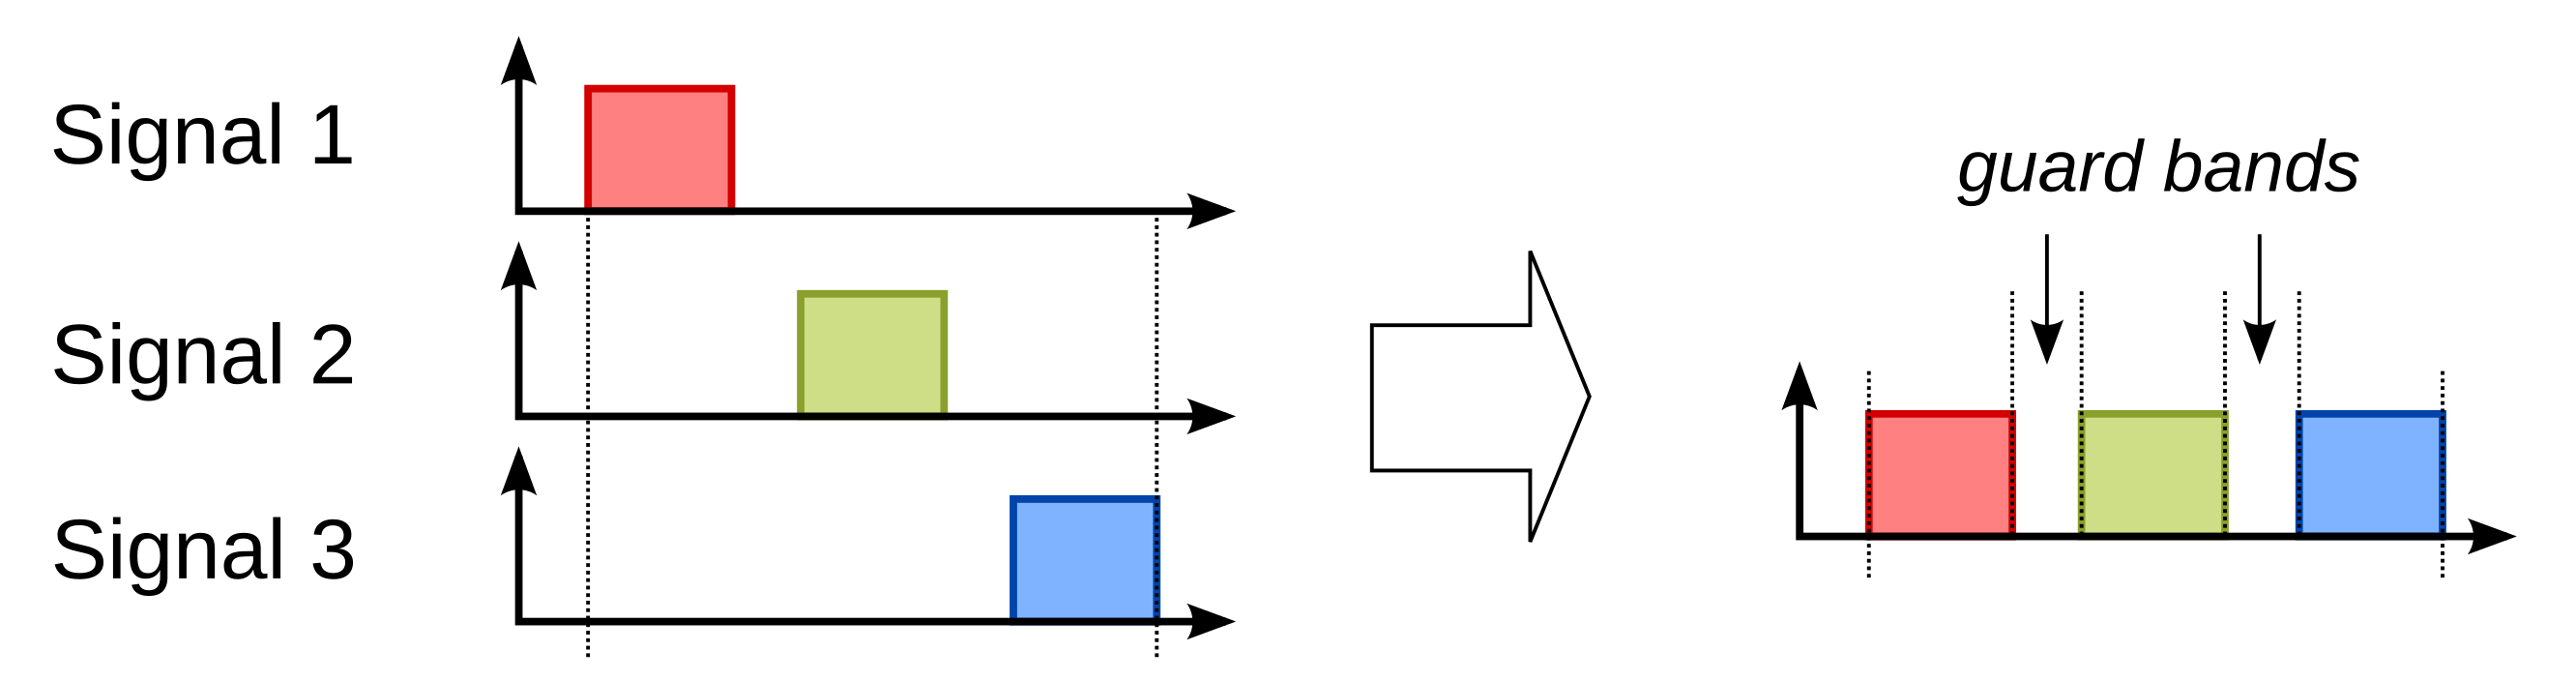
\includegraphics[width=\textwidth]{snimky/TDM.png}}
    \hfill
    \subfloat[Wavelength-division multiplexing (WDM)]{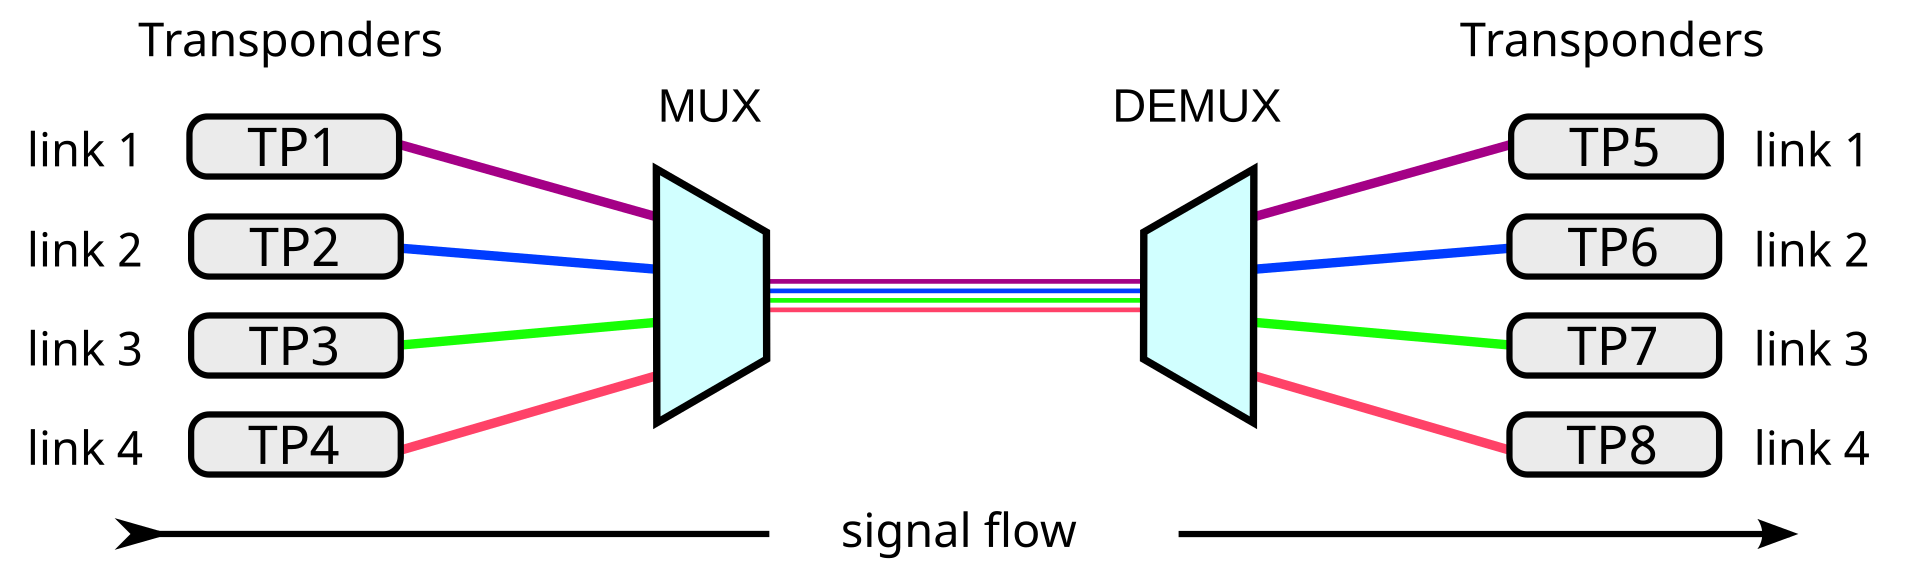
\includegraphics[width=\textwidth]{snimky/WDM.png}}
    \caption{TDM vs. WDM}
\end{figure}

\subsection{Problematika přiřazení vlnových délek (RWA)}
Klasické datové sítě pracují s pakety, které jsou předávány mezi aktivními prvky. Výsledkem je přijetí paketu, kontrola cílové IP adresy a jeho následné odeslání přes zvolené rozhraní. Na druhou stranu optické sítě jsou data přenášená přes optické \enquote{crossconnect}, jenž každý přepíná optický signál, který je přenášen na různé vlnové délce do zvoleného směru.

Pro aplikaci ILP modelu uvažujme následující scénář:
\begin{itemize}
    \item Přiřazování vlnových délek je možné v rozdílných literaturách najít pod problematikou \enquote{barvení grafu}.
    \item Při přiřazování vlnových délek jsou optické trasy vytvářeny na požadavek, kdežto jejich cesty jsou dané předem (tedy fyzickými optickými vlákny mezi prvky)
    \item Pokud dvě trasy sdílí jedno optické vlákno, pak je ustanovena hrana mezi odpovídajícími uzly. V jiném případě nedojde k ustanovení hran, neboť neexistuje sdílené vlákno mezi trasou
    \item Jsou-li dva vrcholy připojeny k hranám, jedná se o sousedy. Vlnové délky odpovídají barvě v grafu
    \item Přiřazení barev v grafu musí splňovat základní podmínku, že stejná barva není přiřazena dvěma sousedícím vrcholům
\end{itemize}
